% !TEX root = ../tex/7-2.tex
% 第7章：本文は青、補足は緑
\newcommand{\asmain}{%
    \setbeamercolor{frametitle}{fg=white,bg=main}%
    \setbeamercolor{structure}{fg=main}%
    \setbeamercolor{itemize item}{fg=main}%
    \setbeamercolor{itemize subitem}{fg=main}%
    \setbeamercolor{enumerate item}{fg=main}%
}
\newcommand{\assuppl}{%
    \setbeamercolor{frametitle}{fg=white,bg=examplecol}%
    \setbeamercolor{structure}{fg=examplecol}%
    \setbeamercolor{itemize item}{fg=examplecol}%
    \setbeamercolor{itemize subitem}{fg=examplecol}%
    \setbeamercolor{enumerate item}{fg=examplecol}%
}
\newcommand{\supplmark}{%
    \setlength{\fboxsep}{1.5pt}%
    \setlength{\fboxrule}{0.7pt}%
    \fbox{\textbf{補足}}%
}
\asmain


%=============================================
\begin{frame}{7.1から7.2へ}
    \begin{block}{ここまで（7.1）}
        分布間翻訳の動機と、\\
        「最も効率的な変換とは／拡散はOTか」という問いを置いた。
    \end{block}
    \begin{block}{ここから（7.2）}
        「最適／効率」の意味を、問題設定の分類として固定する。\\
        古典OT・EOT・Schrödinger bridge・生成モデルとのアナロジー。
    \end{block}
\end{frame}
%=============================================
\asmain
\begin{frame}{7.2 の位置づけ}
    \begin{block}{この節の役割}
        $p_{\mathrm{src}}\to p_{\mathrm{tgt}}$の「安い運び方」を、複数の定式化で整理する
    \end{block}
    \begin{enumerate}
        \item \textbf{7.2.1 古典OT}\\
        カップリング、Monge--Kantorovich、$W_2$、動的BB
        \item \textbf{7.2.2 EOT}\\
        エントロピー正則化とSinkhorn形
        \item \textbf{7.2.3 SB}\\
        経路KL／確率制御、前向き・逆向きSDE
        \item \textbf{7.2.4 アナロジー}\\
        大域プッシュフォワード vs 局所力学
    \end{enumerate}
\end{frame}
%=============================================
\section{7.2.1 Optimal Transport (OT)}
\asmain
\begin{frame}{区切り：7.2.1 Optimal Transport}
    \tableofcontents[currentsection]
\end{frame}
%=============================================
\asmain
\begin{frame}{図7.1：独立カップリングとOTカップリング}
    \centering
    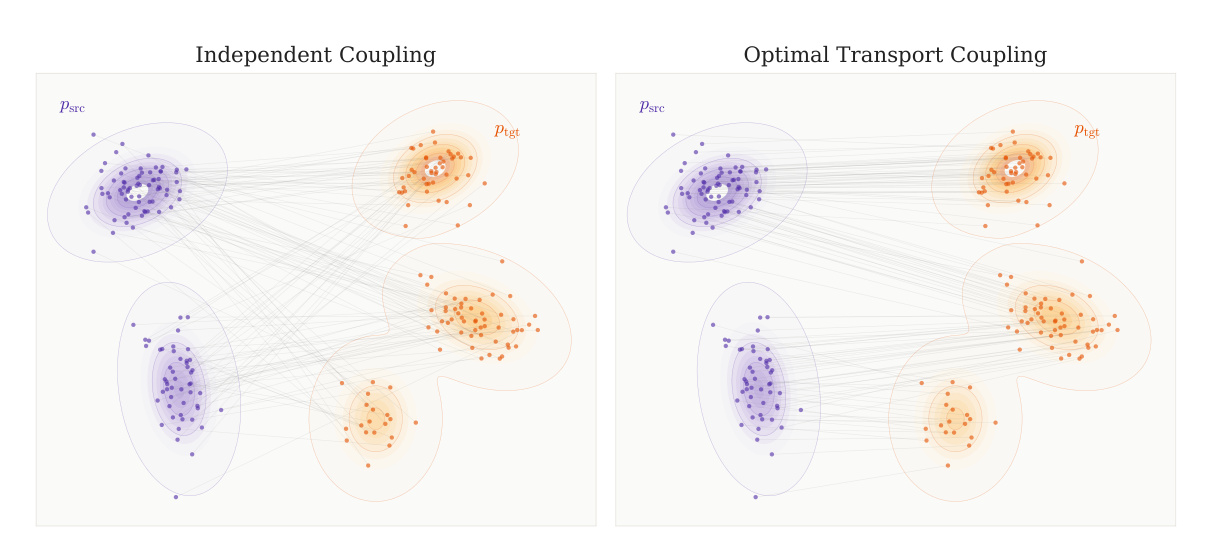
\includegraphics[width=\textwidth,height=0.58\textheight,keepaspectratio]{fig-7-1.jpg}
    \vfill
    \footnotesize
    同じ$p_{\mathrm{src}},p_{\mathrm{tgt}}$でも、対応の取り方で総コストが変わる。\\
    左：独立（交差が多く高い）。右：OT（近い質量同士、交差を避ける）。
\end{frame}
%=============================================
\assuppl
\begin{frame}{\supplmark：図7.1の読み方}
    \begin{columns}[T,onlytextwidth]
        \begin{column}{0.48\textwidth}
            \begin{exampleblock}{独立カップリング}
                実質$\gamma\approx p_{\mathrm{src}}\otimes p_{\mathrm{tgt}}$。\\
                遠い点どうしも結び、\\
                パスが交差しやすい。
            \end{exampleblock}
        \end{column}
        \begin{column}{0.48\textwidth}
            \begin{exampleblock}{OTカップリング}
                期待コストを最小にする対応。\\
                近い質量を優先し、\\
                交差を抑える。
            \end{exampleblock}
        \end{column}
    \end{columns}
    \vspace{0.35em}
    \begin{block}{要点}
        OTの第一歩は「端点分布」ではなく「どの対$(\vx,\bm{y})$を運ぶか」。
    \end{block}
\end{frame}
%=============================================
\asmain
\begin{frame}{カップリングとは}
    コスト$c:\mathbb{R}^{D}\times\mathbb{R}^{D}\to\mathbb{R}$を固定し、\\
    $p_{\mathrm{src}}$を$p_{\mathrm{tgt}}$へできるだけ安く変換したい。
    \begin{itemize}
        \item \textbf{カップリング}$\gamma$：$\mathbb{R}^{D}\times\mathbb{R}^{D}$上の同時分布で、\\
        周辺が$p_{\mathrm{src}}$と$p_{\mathrm{tgt}}$
        \item $(\vx,\bm{y})\sim\gamma$は「ソース点$\vx$をターゲット点$\bm{y}$へ対応付ける」
    \end{itemize}
    密度があるとき周辺制約は
    \[
        \int \gamma(\vx,\bm{y})\,d\bm{y} = p_{\mathrm{src}}(\vx),
        \qquad
        \int \gamma(\vx,\bm{y})\,d\vx = p_{\mathrm{tgt}}(\bm{y}).
    \]
\end{frame}
%=============================================
\asmain
\begin{frame}{カップリングの二例}
    \begin{enumerate}
        \item \textbf{離散サポート}\\
        非負行列$(\gamma_{ij})$で、行和が$p_{\mathrm{src}}$、列和が$p_{\mathrm{tgt}}$。\\
        $\gamma_{ij}$は$i$から$j$へ送る質量。
        \item \textbf{決定写像}\\
        可測写像$T$が$T_{\#}p_{\mathrm{src}}=p_{\mathrm{tgt}}$なら、\\
        $\gamma=(I,T)_{\#}p_{\mathrm{src}}$は各$\vx$を$T(\vx)$へ送る決定カップリング。
    \end{enumerate}
    \begin{exampleblock}{コスト}
        固定$\gamma$の下での輸送コストは
        $\mathbb{E}_{(\vx,\bm{y})\sim\gamma}[c(\vx,\bm{y})]$。
    \end{exampleblock}
\end{frame}
%=============================================
\asmain
\begin{frame}{静的OT：Monge--Kantorovich}
    許容カップリングの中で期待コストを最小化する：
    \[
        \mathrm{OT}(p_{\mathrm{src}},p_{\mathrm{tgt}})
        :=
        \inf_{\gamma\in\Gamma(p_{\mathrm{src}},p_{\mathrm{tgt}})}
        \int c(\vx,\bm{y})\,d\gamma(\vx,\bm{y})
        \tag{7.2.1}
    \]
    実行可能集合は周辺制約のみ：
    \[
        \Gamma(p_{\mathrm{src}},p_{\mathrm{tgt}})
        =
        \bigl\{\gamma\in\mathcal{P}(\mathbb{R}^{D}\times\mathbb{R}^{D}):
        \text{周辺が }p_{\mathrm{src}},p_{\mathrm{tgt}}\bigr\}.
    \]
    \begin{block}{読み}
        「質量保存を守りつつ、最も安い対応$\gamma$を選ぶ」。
    \end{block}
\end{frame}
%=============================================
\asmain
\begin{frame}{特殊例：Wasserstein-2距離}
    二次コスト$c(\vx,\bm{y})=\|\vx-\bm{y}\|_{2}^{2}$のときのOT値が$W_{2}^{2}$：
    \[
        W_{2}^{2}(p_{\mathrm{src}},p_{\mathrm{tgt}})
        :=
        \inf_{\gamma\in\Gamma(p_{\mathrm{src}},p_{\mathrm{tgt}})}
        \mathbb{E}_{(\vx,\bm{y})\sim\gamma}\bigl[\|\vx-\bm{y}\|_{2}^{2}\bigr].
    \]
    Brenierの定理（適当な仮定下）：最適$\gamma$は決定写像$T$のグラフに集中し、
    \[
        W_{2}^{2}(p_{\mathrm{src}},p_{\mathrm{tgt}})
        =
        \inf_{\substack{T:\\T_{\#}p_{\mathrm{src}}=p_{\mathrm{tgt}}}}
        \mathbb{E}_{\vx\sim p_{\mathrm{src}}}\bigl[\|T(\vx)-\vx\|_{2}^{2}\bigr]
        \tag{7.2.2}
    \]
\end{frame}
%=============================================
\assuppl
\begin{frame}{\supplmark：$W_{2}$の三つの顔}
    二次コストでは、次が（正則性の下で）同値：
    \begin{enumerate}
        \item \textbf{Monge}：最適輸送写像$T$
        \item \textbf{Kantorovich}：最適カップリング$\gamma$
        \item \textbf{Benamou--Brenier}：動的な運動エネルギー最小化（次）
    \end{enumerate}
    \begin{exampleblock}{Brenier}
        $p_{\mathrm{src}}$が低次元集合に質量を置かないなら、\\
        最適写像$T_{\star}$が一意に存在する（定理7.1の要旨）。
    \end{exampleblock}
\end{frame}
%=============================================
\asmain
\begin{frame}{動的OT：連続時間の流れ}
    静的な一発写像ではなく、連続時間の密度経路として書く：
    \[
        p_{0}:=p_{\mathrm{src}}
        \;\to\;
        p_{t}
        \;\to\;
        p_{1}:=p_{\mathrm{tgt}},
        \qquad t\in[0,1].
    \]
    Benamou--Brenier（2000）：滑らかな速度場$v_{t}(\vx)$で質量の運動を記述し、\\
    二次コストのOT値を運動エネルギー最小化と同値にする。
\end{frame}
%=============================================
\asmain
\begin{frame}{Benamou--Brenier定式化}
    \[
        \resizebox{0.98\textwidth}{!}{$
        W_{2}^{2}(p_{\mathrm{src}},p_{\mathrm{tgt}})
        =
        \displaystyle\min_{\substack{(p_{t},v_{t}):\\
        \partial_{t}p_{t}+\nabla\cdot(p_{t}v_{t})=0,\\
        p_{0}=p_{\mathrm{src}},\,p_{1}=p_{\mathrm{tgt}}}}
        \displaystyle\int_{0}^{1}\!\int_{\mathbb{R}^{D}}
        \|v_{t}(\vx)\|_{2}^{2}\,p_{t}(\vx)\,d\vx\,dt
        $}
        \tag{7.2.3}
    \]
    \begin{itemize}
        \item 制約は連続方程式（質量保存）と端点条件
        \item 最適流はMcCannの変位補間：
        $T_{t}^{\star}(\vx)=(1-t)\vx+t\,T_{\star}(\vx)$（等速直線）
        \item $p_{t}=T_{t}^{\star}{}_{\#}p_{\mathrm{src}}$
    \end{itemize}
\end{frame}
%=============================================
\asmain
\begin{frame}{図7.2：動的OTのイメージ}
    \centering
    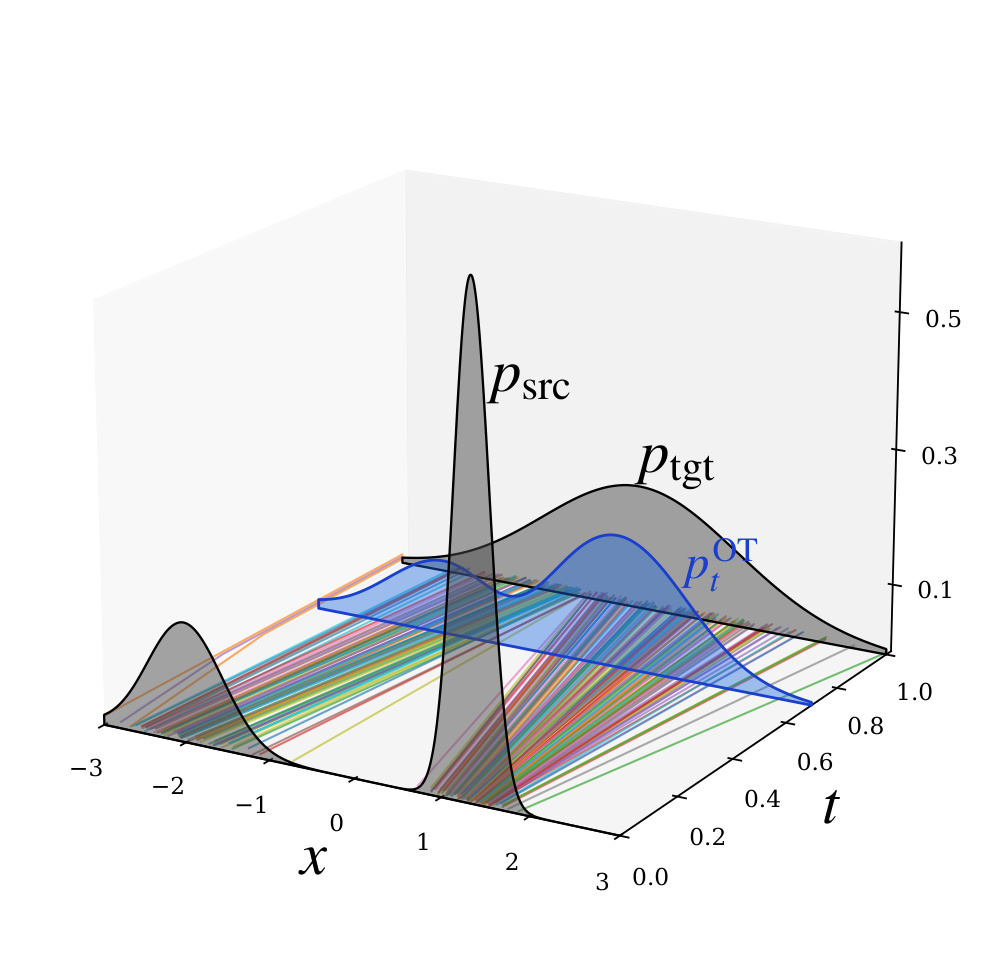
\includegraphics[width=\textwidth,height=0.58\textheight,keepaspectratio]{fig-7-2.jpg}
    \vfill
    \footnotesize
    $p_{t}^{\mathrm{OT}}$は時間連続に進化し、$p_{\mathrm{src}}$を$p_{\mathrm{tgt}}$へ\\
    決定的かつ最小コストで運ぶ（McCann補間）。
\end{frame}
%=============================================
\assuppl
\begin{frame}{\supplmark：図7.2の読み方}
    \begin{itemize}
        \item $t=0$の$p_{\mathrm{src}}$から$t=1$の$p_{\mathrm{tgt}}$へ密度が変形
        \item 中間の$p_{t}^{\mathrm{OT}}$は変位補間の断面
        \item 軌跡は直線・等速（動的$W_{2}$測地線の特徴）
    \end{itemize}
    \begin{exampleblock}{Flow Matchingとの接点}
        「速度場で密度を運ぶ」見た目は近い。\\
        ただし学んだ速度がBB作用を最小化するかは別問題（7.5）。
    \end{exampleblock}
\end{frame}
%=============================================
\asmain
\begin{frame}{Monge--Ampèreと正規化フロー}
    最適写像はBrenierより$T_{\star}(\vx)=\nabla\psi(\vx)$（$\psi$凸）で、
    \[
        p_{\mathrm{tgt}}\bigl(\nabla\psi(\vx)\bigr)\,
        \det\nabla^{2}\psi(\vx)
        =
        p_{\mathrm{src}}(\vx)
        \tag{7.2.4}
    \]
    （Monge--Ampère）。一般に陽に解けない非線形PDE。
    \begin{alertblock}{注意（正規化フローとの差）}
        式(7.2.4)は変数変換関係そのもの。\\
        しかしNFは可逆写像＋扱いやすいJacobianを置くだけで、\\
        一般に$T=\nabla\psi$の構造は課さない$\Rightarrow$Brenier写像とは限らない。
    \end{alertblock}
\end{frame}
%=============================================
\section{7.2.2 Entropy-Regularized OT (EOT)}
\asmain
\begin{frame}{区切り：7.2.2 Entropy-Regularized OT}
    \tableofcontents[currentsection]
\end{frame}
%=============================================
\asmain
\begin{frame}{離散経験測度での動機}
    サンプル$\{x^{(i)}\}$，$\{y^{(j)}\}$に重み$a,b$を載せた経験分布を考える。\\
    カップリングは$n\times n$非負行列$\gamma=(\gamma_{ij})$（行和$a$、列和$b$）。
    \begin{block}{古典OT（離散）}
        \[
            \min_{\gamma}
            \sum_{i,j} C_{ij}\gamma_{ij},
            \qquad
            C_{ij}=c(x^{(i)},y^{(j)}).
        \]
        これは式(7.2.1)の計数測度版（線形計画）。
    \end{block}
\end{frame}
%=============================================
\asmain
\begin{frame}{なぜ正則化するか}
    古典OTの実務上の難点：
    \begin{enumerate}
        \item \textbf{非一意・不安定}\\
        最小コストを達成する計画が複数あり得る。\\
        入力$(a,b,C)$の微小変化で解が跳ねる。
        \item \textbf{計算コスト}\\
        変数$n^{2}$、制約$2n$。\\
        Hungarian／network simplexは概ね$O(n^{3})$で大規模に厳しい。
    \end{enumerate}
    \begin{exampleblock}{方針}
        $\varepsilon>0$のエントロピー項を足し、一意性と計算性を得る。
    \end{exampleblock}
\end{frame}
%=============================================
\asmain
\begin{frame}{EOTの目的関数}
    \[
        \mathrm{EOT}_{\varepsilon}(p_{\mathrm{src}},p_{\mathrm{tgt}})
        :=
        \min_{\gamma\in\Gamma(p_{\mathrm{src}},p_{\mathrm{tgt}})}
        \Biggl(
        \int c\,d\gamma
        +
        \varepsilon\,D_{\mathrm{KL}}(\gamma\|M)
        \Biggr)
        \tag{7.2.5}
    \]
    \begin{itemize}
        \item 参照測度$M$は通常$p_{\mathrm{src}}\otimes p_{\mathrm{tgt}}$
        \item $D_{\mathrm{KL}}(\gamma\|p_{\mathrm{src}}\otimes p_{\mathrm{tgt}})=-H(\gamma)+\mathrm{const}$
        \item $H(\gamma)=-\int\gamma\log\gamma$はShannonエントロピー
    \end{itemize}
\end{frame}
%=============================================
\asmain
\begin{frame}{エントロピー正則化の利点（1/2）}
    \begin{enumerate}
        \item \textbf{質量の拡散}\\
        $\gamma\log\gamma$は尖った計画を罰し、質量をより広く配分する\\
        （エントロピー最大化＝不確かさの増大）
        \item \textbf{強凸と一意性}\\
        $H$の強凹性より式(7.2.5)は$\gamma$について強凸。\\
        最小化子$\gamma_{\varepsilon}^{\star}$は一意で、$(p_{\mathrm{src}},p_{\mathrm{tgt}},c)$に連続依存。
    \end{enumerate}
\end{frame}
%=============================================
\asmain
\begin{frame}{エントロピー正則化の利点（2/2）}
    \begin{enumerate}
        \setcounter{enumi}{2}
        \item \textbf{Schrödinger／Sinkhorn形}\\
        緩和条件の下、
        \[
            \gamma_{\varepsilon}^{\star}(\vx,\bm{y})
            =
            u(\vx)\,e^{-c(\vx,\bm{y})/\varepsilon}\,v(\bm{y})\,
            p_{\mathrm{src}}(\vx)\,p_{\mathrm{tgt}}(\bm{y})
        \]
        （$u,v>0$）。有限サンプルではSinkhorn反復で解ける（概ね反復あたり$O(n^{2})$）。
        \item \textbf{$\varepsilon$の極限}\\
        $\varepsilon\to 0$：古典OTカップリングへ集中。\\
        $\varepsilon$大：独立カップリング$p_{\mathrm{src}}\otimes p_{\mathrm{tgt}}$へ接近。
    \end{enumerate}
\end{frame}
%=============================================
\assuppl
\begin{frame}{\supplmark：EOTの直感まとめ}
    \begin{columns}[T,onlytextwidth]
        \begin{column}{0.48\textwidth}
            \begin{block}{古典OT}
                安いが尖りやすい\\
                解が跳ねる／重い
            \end{block}
        \end{column}
        \begin{column}{0.48\textwidth}
            \begin{block}{EOT}
                コスト＋拡散のトレードオフ\\
                一意・Sinkhorn可能
            \end{block}
        \end{column}
    \end{columns}
    \vspace{0.5em}
    \begin{exampleblock}{次}
        動的・確率過程の言語では、同じ正則化がSchrödinger bridgeになる。
    \end{exampleblock}
\end{frame}
%=============================================
\section{7.2.3 Schrödinger Bridge (SB)}
\asmain
\begin{frame}{区切り：7.2.3 Schrödinger Bridge}
    \tableofcontents[currentsection]
\end{frame}
%=============================================
\asmain
\begin{frame}{SBの問い（経路空間）}
    粒子が単純な参照力学（例：Brown運動）に従うとする。\\
    $t=0$で$p_{\mathrm{src}}$、$t=T$で$p_{\mathrm{tgt}}$を観測したとき：
    \begin{alertblock}{問い}
        両端周辺を満たす確率過程のうち、\\
        参照力学からのずれ（KL）が最小なものは何か？
    \end{alertblock}
    「最も尤もらしい、参照の変形」がSchrödinger bridge。
\end{frame}
%=============================================
\asmain
\begin{frame}{経路法則と周辺}
    \begin{itemize}
        \item 軌跡$x_{0:T}=\{x_{t}\}_{t\in[0,T]}$
        \item $P$：軌跡全体の法則（経路測度）
        \item $p_{t}$（または$P_{t}$）：時刻$t$の周辺（$p_{t}(A)=P(x_{t}\in A)$）
    \end{itemize}
    参照拡散：
    \[
        dx_{t}
        =
        f(x_{t},t)\,dt
        +
        g(t)\,dw_{t}
        \tag{7.2.6}
    \]
    その経路法則を$R$、初期周辺を$R_{0}$と書く。
\end{frame}
%=============================================
\asmain
\begin{frame}{KL定式化のSB}
    \[
        \mathrm{SB}(p_{\mathrm{src}},p_{\mathrm{tgt}})
        :=
        \min_{P}
        D_{\mathrm{KL}}(P\|R)
        \quad\text{s.t.}\quad
        P_{0}=p_{\mathrm{src}},\;
        P_{T}=p_{\mathrm{tgt}}
        \tag{7.2.7}
    \]
    \begin{itemize}
        \item 最適化変数は経路法則$P$
        \item 最小化子$P^{\star}$は参照$R$の取り方に依存
        \item 端点は任意：$R$を両端へ「橋渡し」する
    \end{itemize}
\end{frame}
%=============================================
\asmain
\begin{frame}{確率制御ビュー}
    任意の$P$ではなく、参照にドリフト$v_{t}$を足した制御拡散を候補にする：
    \[
        dx_{t}
        =
        \bigl[f(x_{t},t)+v_{t}(x_{t})\bigr]dt
        +
        g(t)\,dw_{t}.
    \]
    Girsanovの下、
    \[
        D_{\mathrm{KL}}(P\|R)
        =
        D_{\mathrm{KL}}(p_{\mathrm{src}}\|R_{0})
        +
        \frac12
        \mathbb{E}_{P}
        \!\int_{0}^{T}
        \frac{\|v_{t}(x_{t})\|_{2}^{2}}{g^{2}(t)}\,dt.
    \]
    $P_{0}=p_{\mathrm{src}}$固定なら第一項は定数（$R_{0}=p_{\mathrm{src}}$なら0）。
\end{frame}
%=============================================
\asmain
\begin{frame}{確率制御形の目的（式7.2.8）}
    \[
        \resizebox{0.98\textwidth}{!}{$
        \mathrm{SB}(p_{\mathrm{src}},p_{\mathrm{tgt}})
        =
        \displaystyle\min_{\substack{v_{t}:\\
        dx=[f+v]dt+g\,dw,\\
        x_{0}\sim p_{\mathrm{src}},\,x_{T}\sim p_{\mathrm{tgt}}}}
        \displaystyle\frac12
        \int_{0}^{T}\!\int_{\mathbb{R}^{D}}
        \frac{\|v_{t}(\vx)\|_{2}^{2}}{g^{2}(t)}\,
        p_{t}(\vx)\,d\vx\,dt
        $}
        \tag{7.2.8}
    \]
    \begin{exampleblock}{読み}
        参照に近い制御エネルギーで、両端周辺へ舵取りする。
    \end{exampleblock}
\end{frame}
%=============================================
\asmain
\begin{frame}{図7.3：SBの確率制御ビュー}
    \centering
    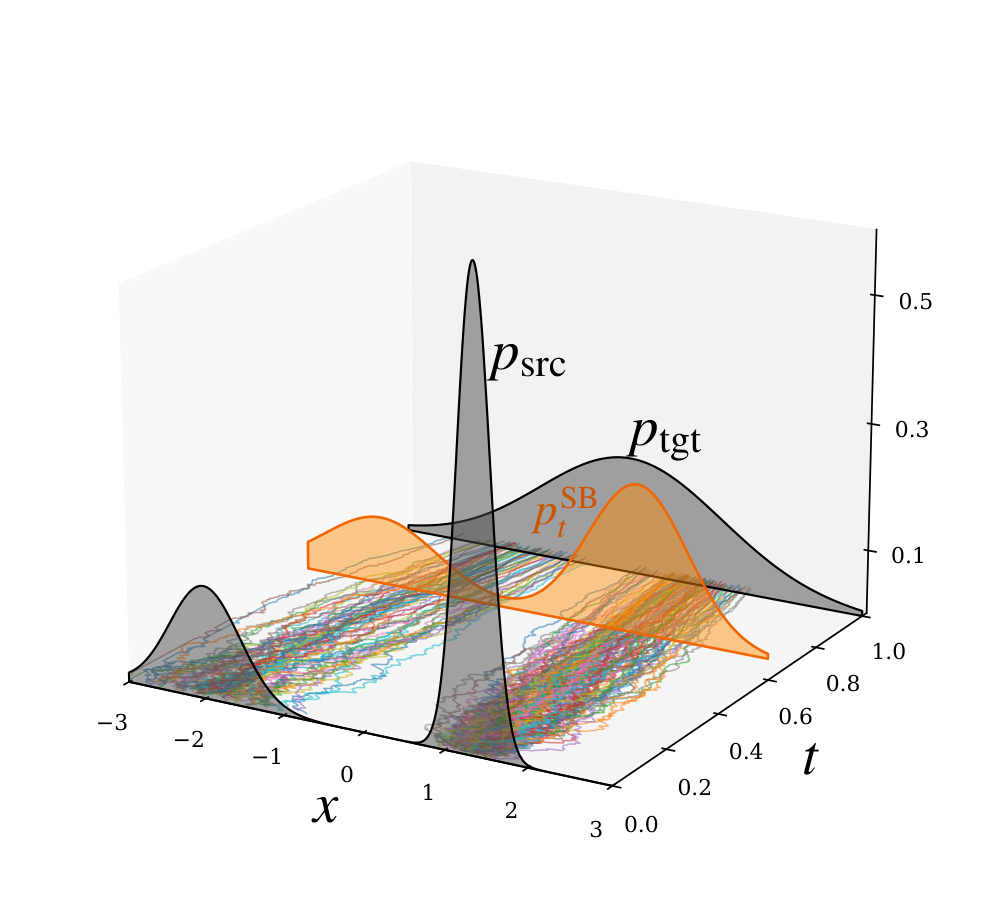
\includegraphics[width=\textwidth,height=0.58\textheight,keepaspectratio]{fig-7-3.jpg}
    \vfill
    \footnotesize
    参照からのずれが最小な確率経路で$p_{\mathrm{src}}$と$p_{\mathrm{tgt}}$を結ぶ。\\
    軌跡は拡散的（OTの直線とは対照的）。
\end{frame}
%=============================================
\assuppl
\begin{frame}{\supplmark：図7.2と図7.3の対比}
    \begin{columns}[T,onlytextwidth]
        \begin{column}{0.48\textwidth}
            \begin{block}{図7.2（OT）}
                決定的・直線軌跡\\
                連続方程式\\
                運動エネルギー最小
            \end{block}
        \end{column}
        \begin{column}{0.48\textwidth}
            \begin{block}{図7.3（SB）}
                確率的・揺らぎあり\\
                Fokker--Planck\\
                参照KL／制御エネルギー最小
            \end{block}
        \end{column}
    \end{columns}
    \vspace{0.4em}
    \begin{exampleblock}{共通点}
        どちらも「時間付きの運び方」を最適化する動的視点。
    \end{exampleblock}
\end{frame}
%=============================================
\asmain
\begin{frame}{特殊例：Brown参照}
    $f\equiv 0$、$g(t)\equiv\sqrt{\varepsilon}$、すなわち
    \[
        dx_{t}=\sqrt{\varepsilon}\,dw_{t}
    \]
    のとき、
    \[
        \mathrm{SB}_{\varepsilon}(p_{\mathrm{src}},p_{\mathrm{tgt}})
        :=
        \min_{P}
        D_{\mathrm{KL}}(P\|R_{\varepsilon})
        \quad\text{s.t.}\quad
        P_{0}=p_{\mathrm{src}},\;
        P_{T}=p_{\mathrm{tgt}}
        \tag{7.2.9}
    \]
    制御形は
    \[
        \min_{v}
        \frac{1}{2\varepsilon}
        \int_{0}^{T}\!\int \|v_{t}\|_{2}^{2}\,p_{t}\,d\vx\,dt
        \quad
        (dx=v\,dt+\sqrt{\varepsilon}\,dw)
        \tag{7.2.10}
    \]
\end{frame}
%=============================================
\assuppl
\begin{frame}{\supplmark：BBとの類似とFisher項}
    式(7.2.10)は見た目がBenamou--Brenier（7.2.3）に近い。\\
    時間対称の流体形では、Brown参照SBは概ね
    \[
        \int\!\!\int
        \Bigl(
        \tfrac12\|\tilde{v}_{t}\|_{2}^{2}
        +
        \tfrac{\varepsilon^{2}}{8}\|\nabla\log\rho_{t}\|_{2}^{2}
        \Bigr)
        \rho_{t}\,d\vx\,dt
    \]
    （運動エネルギー＋Fisher情報）と書ける。
    \begin{exampleblock}{含意}
        二次コスト＋Brown参照では、EOT／SBは\\
        動的OTのFisher正則化版と見なせる（Chen et al., 2021）。
    \end{exampleblock}
\end{frame}
%=============================================
\asmain
\begin{frame}{なぜ参照分布が必要か}
    \begin{columns}[T,onlytextwidth]
        \begin{column}{0.48\textwidth}
            \begin{block}{古典OT}
                地上コスト$c(\vx,\bm{y})$が\\
                「対の高さ」を直接与える。\\
                参照経路は不要。
            \end{block}
        \end{column}
        \begin{column}{0.48\textwidth}
            \begin{block}{SB}
                比較対象が端点対ではなく\\
                \textbf{軌跡全体}。\\
                非制御時の標準挙動として$R$が要る。
            \end{block}
        \end{column}
    \end{columns}
    \vspace{0.4em}
    $D_{\mathrm{KL}}(P\|R)$は、端点制約を満たすために\\
    参照力学からどれだけ外れるかを測る。
\end{frame}
%=============================================
\asmain
\begin{frame}{結合PDEによる特徴付け}
    最適経路の周辺$p_{t}^{\mathrm{SB}}$はポテンシャル分解
    \[
        p_{t}^{\mathrm{SB}}(\vx)
        =
        \Psi(\vx,t)\,\widehat{\Psi}(\vx,t)
        \tag{7.2.11}
    \]
    を持ち、$\Psi,\widehat{\Psi}$は線形Schrödinger系（要旨）：
    \[
        \partial_{t}\Psi
        =
        -\nabla\Psi\cdot f
        -
        \tfrac{g^{2}(t)}{2}\Delta\Psi,
        \quad
        \partial_{t}\widehat{\Psi}
        =
        -\nabla\cdot(\widehat{\Psi}f)
        +
        \tfrac{g^{2}(t)}{2}\Delta\widehat{\Psi}
        \tag{7.2.12}
    \]
    端点：$\Psi\widehat{\Psi}|_{t=0}=p_{\mathrm{src}}$、$\Psi\widehat{\Psi}|_{t=T}=p_{\mathrm{tgt}}$。
\end{frame}
%=============================================
\asmain
\begin{frame}{前向きSB-SDE}
    $\Psi$が分かれば、最適ダイナミクスは参照を$\Psi$で傾ける：
    \[
        dx_{t}
        =
        \bigl[
        f(x_{t},t)
        +
        g^{2}(t)\nabla\log\Psi(x_{t},t)
        \bigr]dt
        +
        g(t)\,dw_{t},
        \quad
        x_{0}\sim p_{\mathrm{src}}
        \tag{7.2.13}
    \]
    制御の最小化子は
    \[
        v_{t}^{\star}(\vx)=g^{2}(t)\nabla_{\vx}\log\Psi(\vx,t).
    \]
    これが端点を合わせる最小KL摂動。
\end{frame}
%=============================================
\asmain
\begin{frame}{逆時間SB-SDE}
    同じ最適経路法則は逆時間でも生成できる：
    \[
        dx_{t}
        =
        \bigl[
        f(x_{t},t)
        -
        g^{2}(t)\nabla\log\widehat{\Psi}(x_{t},t)
        \bigr]dt
        +
        g(t)\,d\bar{w}_{t},
        \quad
        x_{T}\sim p_{\mathrm{tgt}}
        \tag{7.2.14}
    \]
    \begin{itemize}
        \item 時間反転の恒等式$b^{-}=b^{+}-g^{2}\nabla\log p_{t}^{\mathrm{SB}}$から導出
        \item 前向きの$g^{2}\nabla\log\Psi$と逆向きの$-g^{2}\nabla\log\widehat{\Psi}$が制御力
        \item 周辺は常に$p_{t}^{\mathrm{SB}}$
    \end{itemize}
\end{frame}
%=============================================
\assuppl
\begin{frame}{\supplmark：結合PDEの実務的障壁}
    生成に式(7.2.14)を使うには$\widehat{\Psi}$が必要だが、\\
    結合PDE（7.2.12）は低次元でも解くのが難しい。
    \begin{exampleblock}{代替戦略（論文が挙げる例）}
        \begin{itemize}
            \item Score SDEで半橋を反復（De Bortoli et al., 2021）
            \item 代理尤度境界の最適化（Chen et al., 2022; Liu et al., 2023）
            \item $(x_{0},x_{T})$条件付きの解析事後に基づくシミュレーションフリー学習
        \end{itemize}
        詳細は7.4の拡散--SB接続へ。
    \end{exampleblock}
\end{frame}
%=============================================
\section{7.2.4 大域写像と局所力学}
\asmain
\begin{frame}{区切り：7.2.4 大域写像と局所力学}
    \tableofcontents[currentsection]
\end{frame}
%=============================================
\asmain
\begin{frame}{OT視点での生成モデル}
    静的OT（7.2.1）の言葉では、深層生成は
    \[
        G_{\phi}{}_{\#}p_{\mathrm{prior}}
        \approx
        p_{\mathrm{data}}
    \]
    というプッシュフォワード写像の学習と読める。
    \begin{itemize}
        \item 一般に$G_{\phi}$は最適輸送写像とは一致しない
        \item OT目的を陽に課す研究もあるが、例外的
    \end{itemize}
    \begin{block}{動的視点（7.2.3）}
        一枚の大域写像ではなく、時間依存の局所ベクトル場が\\
        $p_{\mathrm{prior}}$と$p_{\mathrm{data}}$の間の滑らかな経路を描く。
    \end{block}
\end{frame}
%=============================================
\asmain
\begin{frame}{静的$\leftrightarrow$動的の並行構造}
    \begin{center}
    \begin{tabular}{lll}
        \hline
        & 静的（大域） & 動的（局所） \\
        \hline
        OT & カップリング／写像 & Benamou--Brenier速度場 \\
        SB & 経路KL（7.2.7） & 確率制御（7.2.8） \\
        DGM & GAN／VAEの$G_{\phi}$ & 拡散の時間依存場 \\
        \hline
    \end{tabular}
    \end{center}
    \vspace{0.6em}
    \begin{exampleblock}{アナロジー}
        GAN／VAE $\approx$ 大域プッシュフォワード。\\
        拡散 $\approx$ 局所力学（速度／スコア／ドリフト）の学習。
    \end{exampleblock}
\end{frame}
%=============================================
\asmain
\begin{frame}{7.2が残すメッセージ}
    \begin{itemize}
        \item 「最適」は問題設定（静的／動的／エントロピー／参照）で意味が変わる
        \item EOTとSBは同じ正則化思想の静的・動的な顔
        \item 拡散モデルの見た目は動的OT／SBに近いが、\\
        \textbf{実際にその最適解か}は7.4--7.5で別途問う
    \end{itemize}
    \begin{block}{次（7.3）}
        OT／EOT／SBの定式化どうしの関係図（図7.4）を精密化する。
    \end{block}
\end{frame}
%=============================================
\section{まとめ}
\asmain
\begin{frame}{区切り：7.2のまとめ}
    \tableofcontents[currentsection]
\end{frame}
%=============================================
\asmain
\begin{frame}{7.2 全体のまとめ}
    \begin{enumerate}
        \item \textbf{OT}
        カップリング上の期待コスト最小化（7.2.1）。$W_{2}$は二次コスト
        \item \textbf{動的OT}
        BB作用（7.2.3）とMcCann直線補間。図7.2
        \item \textbf{EOT}
        $\varepsilon$KL正則化（7.2.5）。一意・Sinkhorn・$\varepsilon$極限
        \item \textbf{SB}
        参照への経路KL最小（7.2.7）／制御形（7.2.8）。図7.3
        \item \textbf{アナロジー}
        大域写像（GAN等）vs 局所場（拡散）
    \end{enumerate}
\end{frame}
%=============================================
\asmain
\begin{frame}{7.2 全体のまとめ：一本の流れ}
    \begin{block}{今日の道筋}
        カップリング
        $\;\to\;$
        $W_{2}$／BB
        $\;\to\;$
        EOT
        $\;\to\;$
        SB（制御・PDE）
        $\;\to\;$
        DGMアナロジー
    \end{block}
    \begin{block}{核心}
        分布間翻訳の「安さ」は、静的対応・決定流・制御拡散で定義が分岐する。\\
        拡散はその言語で読めるが、最適性は自動ではない。
    \end{block}
    \begin{block}{次へ（7.3）}
        EOT$\leftrightarrow$SB、$\varepsilon\to 0$で古典OTへ戻る関係を整理する。
    \end{block}
\end{frame}
